\documentclass[10pt]{article}
\usepackage{icmlko}

\icmlmeta{IP 파운데이션 월드모델}{164}{같은 이름, 다른 물건}{장소 노출과 입장 마찰이 왜 71\%인지 물었다. 코드를 읽어 보니 ``장소 노출''은 열 도메인 중 일곱에서 장소가 아니라 제작사의 사전 출시작 수였다}

\begin{document}

\twocolumn[
\icmlheader

\begin{abstract}
노트 163이 ``장소 노출 74\% · 입장 마찰 68\% --- 교란인가 정의인가''를
남겼다. 교란을 찾는 대신 \texttt{ingest/*\_axes.py} 열 개를 읽었다.
\textbf{정의였다, 그리고 생각보다 심하다.} \texttt{venue\_prominence} 는
팝업에서 매장 내 물리적 위치 노출도인데, \textbf{만화 · 세계애니 · 모바일 ·
도서 · 펀딩 · 아이돌 · 게임 일곱에서는 ``제작사/개발사의 사전 출시작
수''}이고 애니에서는 스튜디오 수, 웹툰에서는 연재 요일 수다.
\textbf{슬롯 이름이 틀렸다} --- 열 중 일곱에서 이 축은 장소가 아니라
\emph{제작 주체의 이력}이다. \texttt{entry\_friction} 도 넷이다: 팝업의
입장 허들, 다섯 도메인의 가격, 웹툰의 유료 회차, 그리고 만화 · 세계애니의
\textbf{성인물 여부}. 반대로 손잡이가 되는 두 축은 구성물이 하나다 ---
\texttt{target\_breadth} 는 태그 수 · 언어 수 · 연령 폭으로 전부 ``얼마나
많은 부류에 닿나''이고, \texttt{goods\_scale} 은 회차 · 분량 · 용량 ·
리워드 수로 전부 ``얼마나 많이 담겼나''다. 나란히 놓으면
\textbf{구성물 하나짜리 둘이 100\% · 98\%, 넷~다섯짜리 셋이
68$\sim$75\%}다(순위상관 $-$0.632). \textbf{다만 인과는 못 가른다} ---
구성물이 많은 축은 효과도 작아서 노트 163의 크기 설명($+$0.900)과 얽힌다.
가르는 사례가 하나 있다: \textbf{미디어 푸시는 효과가 0.042로 큰 축에
가까운데 구성물이 다섯이고 정확도가 75\%다.} 크기만이 설명이라면 95\%
언저리여야 한다. 표본이 축 하나라 확정은 못 하지만 방향은 그쪽이다.
남기는 것은 문서다 --- \texttt{docs/AXIS\_MEANING.md} 에 슬롯마다 도메인별
실제 구성물을 적었다. \textbf{160노트 동안 ``공통 축 다섯''이라 불러 온
것이 실은 슬롯 다섯이었다.}
\end{abstract}
]

\begin{figure*}[t]
\centering
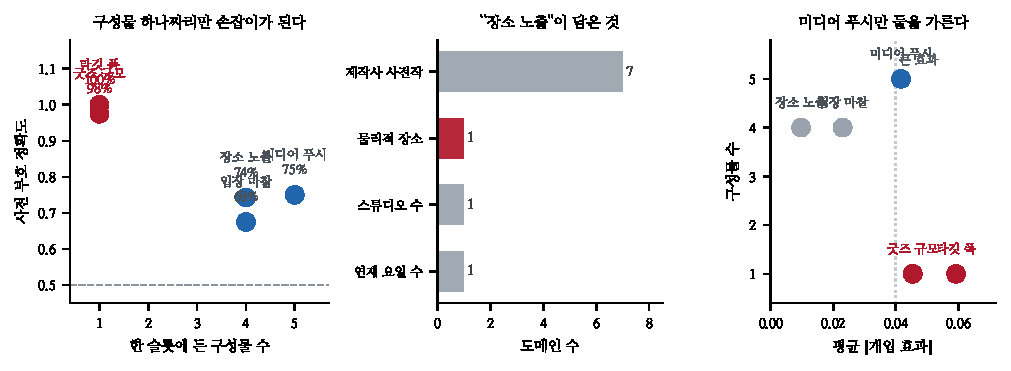
\includegraphics[width=\textwidth]{figs/slot.pdf}
\caption{왼쪽 --- 구성물 하나짜리만 손잡이가 된다. 가운데 --- ``장소
노출''이 실제로 담은 것. 오른쪽 --- 미디어 푸시만 크기와 구성물을 가른다.}
\end{figure*}

\section{장소 노출이 장소가 아니다}

\begin{table}[t]
\centering\tsize
\caption{\texttt{venue\_prominence} 가 도메인마다 재는 것.}
\begin{tabular}{lr}
\toprule
\textbf{제작사·개발사 사전 출시작 수} & \textbf{7} \\
매장 내 물리적 위치 (팝업) & 1 \\
스튜디오 수 (애니) & 1 \\
연재 요일 수 (웹툰) & 1 \\
\bottomrule
\end{tabular}
\end{table}

\claimx{\textbf{슬롯 이름이 틀렸다.} 열 중 일곱에서 이 축은 장소가 아니라
제작 주체의 이력이다 --- \texttt{mobile\_axes.py} 의 주석이 그대로
``개발사 사전 출시 $n$건''이라 적고 있다.}{배선한 쪽에서 속인 것이 아니다.
노트 28 · 40이 ``쌍별 정렬이 도메인별 관측 차이를 허용한다''고 정해 뒀고,
그 아래에서는 슬롯에 무엇을 넣든 정렬이 회전으로 맞춘다고 봤다.
\textbf{직접 풀링으로 바꾼 노트 125 이후 그 전제가 깨졌는데 배선은
그대로였다.}}

\begin{table}[t]
\centering\tsize
\caption{\texttt{entry\_friction} 도 넷이다.}
\begin{tabular}{lr}
\toprule
가격 (애니 · 모바일 · 도서 · 펀딩 · 아이돌) & 5 \\
\textbf{성인물 여부} (만화 · 세계애니) & \textbf{2} \\
입장 허들 (팝업) & 1 \\
유료 회차 (웹툰) & 1 \\
\bottomrule
\end{tabular}
\end{table}

\section{되는 축은 구성물이 하나다}

\begin{table}[t]
\centering\tsize
\caption{손잡이가 되는 두 축.}
\begin{tabular}{ll}
\toprule
\textbf{타깃 폭} & 태그 수 · 언어 수 · 연령 폭 · 후원자 폭 \\
& $\to$ 전부 ``얼마나 많은 부류에 닿나'' \\
\midrule
\textbf{굿즈 규모} & 주당 회차 · 총 분량 · 앱 용량 · 디스크 \\
& 용량 · 양장본 · 리워드 단계 · 수록곡 \\
& $\to$ 전부 ``얼마나 많이 담겼나'' \\
\bottomrule
\end{tabular}
\end{table}

\begin{table}[t]
\centering\tsize
\caption{나란히 놓으면.}
\begin{tabular}{lrrr}
\toprule
& 구성물 & 부호 정확 & 평균 $|$효과$|$ \\
\midrule
\textbf{타깃 폭} & \textbf{1} & \textbf{100\%} & .0593 \\
\textbf{굿즈 규모} & \textbf{1} & \textbf{98\%} & .0454 \\
미디어 푸시 & 5 & 75\% & .0417 \\
장소 노출 & 4 & 74\% & .0097 \\
입장 마찰 & 4 & 68\% & .0230 \\
\bottomrule
\end{tabular}
\end{table}

\claimx{\textbf{구성물 하나짜리만 손잡이가 된다.} 순위상관 $-$0.632이고,
사실상 두 무리다 --- 하나짜리 둘이 99\%, 넷$\sim$다섯짜리 셋이
68$\sim$75\%.}{축이 다섯뿐이라 순위상관의 표준오차가 크다. 무리 사이 격차
(99\% 대 71\%)가 크다는 것이 근거다.}

\section{인과는 못 가른다 --- 하나만 빼고}

\claimx{\textbf{구성물 수와 효과 크기가 얽혀 있다.} 노트 163이 크기와
정확도의 순위상관 $+$0.900을 쟀는데, 구성물이 많은 축은 대개 효과도 작다.
둘 중 무엇이 원인인지 축 다섯으로는 안 갈린다.}{자연스러운 이야기이기도
하다 --- 여러 구성물을 한 슬롯에 넣으면 서로 상쇄돼 효과가 작아진다. 그러면
구성물이 원인이고 크기가 결과다. 반대 방향도 가능하다.}

\claimx{\textbf{미디어 푸시가 유일한 분리 사례다.} 효과가 0.0417로 굿즈
규모(0.0454)와 거의 같은데 정확도는 75\%다. 크기만이 설명이라면 95\%
언저리여야 한다.}{축 하나짜리 증거다. 게다가 미디어 푸시는 칸이 넷뿐이라
75\%의 표준오차가 크다(노트 163). \textbf{방향은 그쪽이지만 확정은 아니다.}}

\section{남기는 것}

\texttt{docs/AXIS\_MEANING.md} 에 슬롯 다섯 $\times$ 도메인 열의 실제
구성물을 적었다. 노트 140이 ``축 이름이 도메인을 건너 같은 뜻인가''를 묻고
\texttt{venue\_prominence} 를 $4/7$ · $|r|{=}0.12$ 로 지목했는데, 그때는
자료로만 봤다. 이번엔 코드로 확인했다.

\claimx{\textbf{규약: 새 도메인에 축을 배선할 때 슬롯 이름이 아니라
구성물을 맞춘다.} 맞출 수 없으면 관측 없음으로 둔다 --- 억지로 채우면
슬롯이 평균을 흐린다.}{지금 배선을 되돌리자는 말은 아니다. 되돌리면
\texttt{venue\_prominence} 가 일곱 도메인에서 사라져 판이 어떻게 될지
모른다. \textbf{그건 재 볼 일이고, 이 노트는 무엇이 들어 있는지까지다.}}

\begin{table}[t]
\centering\tsize
\caption{남은 것.}
\begin{tabular}{ll}
\toprule
\textbf{되돌리면} & 장소 노출을 일곱에서 빼면 판이 어떻게 되나 \\
새 슬롯 & ``제작사 이력''을 여섯째 축으로 분리하면 \\
미디어 푸시 & 구성물 다섯 --- 하나로 좁히면 오르나 \\
\bottomrule
\end{tabular}
\end{table}

둘째 줄이 제일 값질 것 같다. ``제작사/개발사 사전 출시작 수''는 일곱
도메인이 이미 공유하는 진짜 공통 구성물이다. 장소 노출 슬롯에 세 들어
있을 것이 아니라 \textbf{여섯째 축으로 따로 세우면} 구성물 하나짜리 축이
셋이 된다.

\end{document}
